\chapter{Datenbanken}
Im Rahmen dieses Kapitels zwei unterschiedliche Arten von \acl{dbms} erläutert. Zu diesen Arten gehören \acl{rdbms}, \acl{ddbms} und \acl{gdbms}. Im Zuge der Erläuterung der \acs{dbms} werden das Modell, die Geschichte sowie besondere Eigenschaften angesprochen. Ziel ist es dabei nicht die Modelle ausführlich bis in das kleinste Detail zu erklären. Stattdessen soll im Rahmen dieses Kapitels lediglich die grobe Herkunft, das Modell und die Funktionsweise der verschiedenen \acs{dbms}-Konzepte erläutert werden, sodass in den folgenden Kapiteln auf den hier beschriebenen Begriffen und Konzepten aufgebaut werden kann.   

\section{\acl{rdbms}s}
Bei dem relationalen Datenbankmanagementsystemen handelt es sich um eine verbreitetet und erprobte Art \acs{dbms}. Schließlich solche relationalen Systeme bereits seit einigen Jahren am Markt verfügbar. 

\subsection{Geschichte}
Das relationale Datenmodell auf dem alle relationalen Datenbankmanagementsysteme aufbauen, hat seinen Ursprung in den 1970er Jahren. Dort wurde es erstmals in \cite{codd_relational_model} beschrieben. Im Rahmen von \cite{codd_relational_model} umreist \citeauthor{codd_relational_model} ein Datenmodell, bei dem Informationen in Form von Tupeln und Relationen organisiert werden. Angelehnt an das von \citeauthor{codd_relational_model} skizzierte Datenmodell, wurden in den folgenden Jahren die ersten relationalen Datenbanksysteme entwickelt. 

\subsection{Modell}
Relationale Datenbanksysteme organisieren hierbei ihre Daten in Form von Tabellen (Relationen), Spalten und Zeilen (Tupeln). Tabellen stellen dabei immer einen bestimmten Entitätentyp dar z.B. ein Auto oder einen Autobesitzer. Diese Entitätentypen verfügen immer über ein oder mehrere fest definierte Attribute. Bei einem Auto könnten solche Attribute die Fahrzeugnummer, der Marke, das Modell und das Baujahr sein, siehe \autoref{tab:auto_table}. 

\begin{table}[h]
    \centering
    \begin{tabular}{c|c|c|c}
    \hline
    \rowcolor[HTML]{EFEFEF} 
    \multicolumn{1}{l|}{\cellcolor[HTML]{EFEFEF}\textbf{Fahrzeugnummer}} & \multicolumn{1}{l|}{\cellcolor[HTML]{EFEFEF}\textbf{Marke}} & \multicolumn{1}{l|}{\cellcolor[HTML]{EFEFEF}\textbf{Model}} & \multicolumn{1}{l}{\cellcolor[HTML]{EFEFEF}\textbf{Baujahr}} \\ \hline
    FZ-123456789 & Toyota & Starlet & 1997 \\
    FZ-234567890 & Nissan & Leaf & 2018 \\
    FZ-345678912 & VW & ID3 & 2020 \\
    FZ-456789123 & Ford & Fiesta & 2001 \\
    ... & ... & ... & ... \\ \hline
    \end{tabular}
    \caption{Auto Tabelle}
    \label{tab:auto_table}
\end{table}

Es ist dabei auch möglich, Beziehungen zwischen unterschiedlichen Entitätentypen (Tabellen) aufzubauen. Hierbei unterstützen relationale Datenbanksysteme die folgenden Typen von Entitätsbeziehungen: 
\begin{itemize}
    \item \textit{one-to-one}, 
    \item \textit{one-to-many} bzw. \textit{many-to-one} und 
    \item \textit{many-to-many}.
\end{itemize}
\textit{One-to-one}- und \textit{one-to-many}-Beziehungen lassen sich dabei ohne großen Aufwand umsetzen. Hierbei muss lediglich eine neue Spalte für Fremdschlüssel in eine der Tabellen eingefügt werden. Dieser verweist auf das identifizierende Attribut -- den Primärschlüssel -- der anderen Tabelle. Die Abstraktion von \textit{many-to-many}-Beziehungen ist hierbei etwas aufwändiger. Dabei muss eine Auflösungstabelle zwischen den zwei Tabellen aufgebaut werden, deren Entitätstypen in einer \textit{many-to-many}-Beziehung stehen. So wäre es beispielsweise möglich eine Besitz-Beziehung zwischen Autos und allen aktuellen und ehemaligen Besitzern aufzubauen. Diese Auflösungstabelle könnte dabei in Form eines Kfz-Registers abstrahiert werden, siehe \autoref{fig:rdbms_m2m}.

\begin{figure}[h]
    \centering
    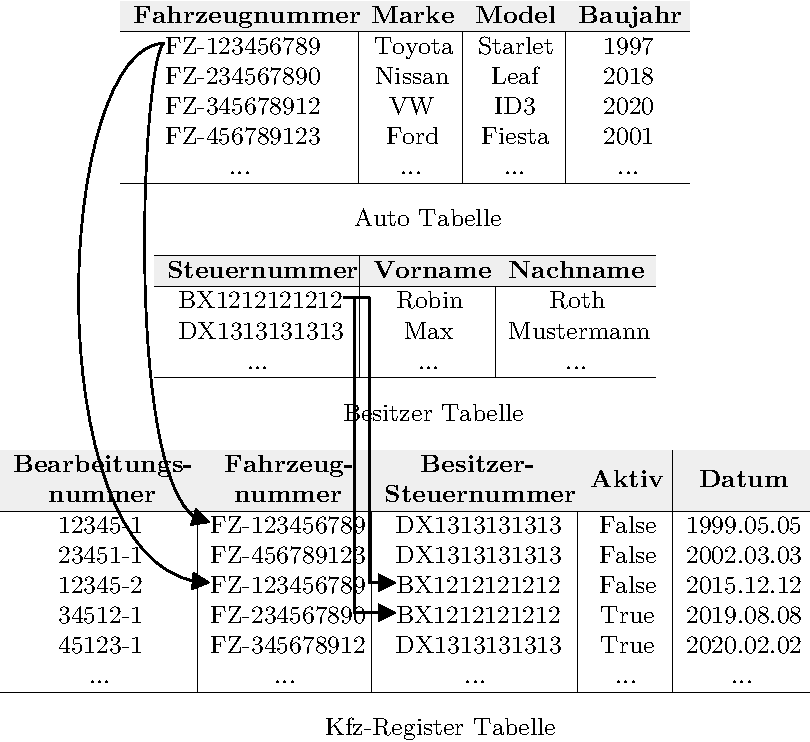
\includegraphics[width=\textwidth]{images/many-to-many.pdf}
    \caption{Beispiel RDBMS many-to-many-Beziehungen}
    \label{fig:rdbms_m2m}
\end{figure}

\subsection{SQL}
Über das Konzept des relationale Konzept der Datenbanken hinaus, gilt es die Abfragesprache SQL herauszustellen. Die Abfragesprache wurde als relationale Sprachen entworfen \cite{sql_history}. Dies geschah in Reaktion auf das von \citeauthor{codd_relational_model} beschriebene relationale Modell \cite{sql_history}. Darüber hinaus gilt nach \cite{sql_history} SQL als eine einfach zu erlernende Sprache. 

SQL nimmt heute im Umfeld von \acs{rdbms} eine große Rolle ein. Bekannte relationale Datenbanksysteme wie DB2, PostgreSQL, Oracle Database und Microsoft SQL Server unterstützen alle die Abfragesprache SQL. Einige von den aufgeführten Systemen tragen die Abfragesprache sogar im Namen. Dabei gilt es allerdings zu beachten, dass sich die angesprochenen Datenbanksysteme alle durch verschiedene SQL-Dialekte auszeichnen. 

Die SQL als relationale Sprache ermöglicht es Datenstrukturen in Form von Tabelle zu definieren. Für das Schreiben der Daten in die Tabelle sowie das Auslesen, Ändern und Löschen bietet SQL ebenfalls Operationen an. Mit Primär- und Fremdschlüssel verfügt der SQL-Sprachumfang auch über Konstrukte zur Abbildung von Entitätsbeziehungen. 

\section{\acl{gdbms}s}



